\documentclass{article}
\usepackage[utf8]{inputenc}
\usepackage{tikz}
\usepackage{ifthen}
\usepackage[top=4cm,bottom=3cm,left=3cm,right=3cm]{geometry}
\usetikzlibrary{automata}
\newboolean{sol}
\newboolean{ex}
\setboolean{ex}{true}
\setboolean{sol}{true}

\usepackage{float}
\begin{document}
\title{Übungsaufgaben}
\author{Simon Stroh und Moritz von Looz}
\maketitle
\section{Endliche Automaten}
\ifthenelse{\boolean{ex}}{
\subsection{Aufgaben}
Gegeben sei folgender nichtdeterministischer endlicher Automat:
\begin{center}
\begin{figure}[H]
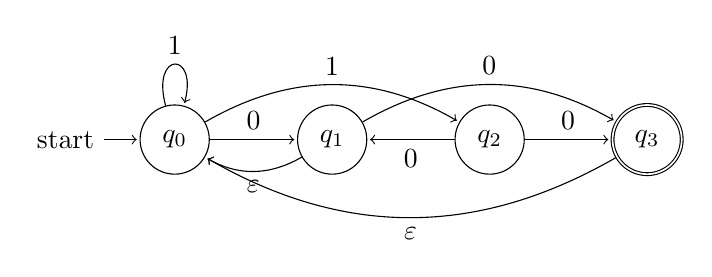
\begin{tikzpicture}[node distance=2cm,shorten >=1pt,auto]
\node[state,initial] 	(q_0)			{$q_0$};
\node[state]		(q_1)	[right of=q_0]	{$q_1$};
\node[state]		(q_2)	[right of=q_1]	{$q_2$};
\node[state,accepting]	(q_3)	[right of=q_2]	{$q_3$};
\path[->]		(q_0)	edge 			node	{$0$}		(q_1)
				edge [bend left]	node	{$1$}		(q_2)
				edge [loop above]	node	{$1$}		()
			(q_1)	edge [bend left]	node	{$\varepsilon$}	(q_0)
				edge [bend left]	node	{$0$}		(q_3)
			(q_2)	edge 			node	{$0$}		(q_1)
				edge			node	{$0$}		(q_3)
			(q_3)	edge [bend left]	node	{$\varepsilon$}	(q_0);
\end{tikzpicture}
\end{figure}
\end{center}
\begin{enumerate}
\item Bilde einen äquivalenten, minimalen DEA.
\item Was sind die Äquivalenzklassen für diesen Automaten bezüglich der Nerode-Relation?
\item Bilde einen regulären Ausdruck der die gleiche Sprache akzeptiert wie der Automat.
\item Folgt aus $L$ regulär das $L^R$ regulär ist? (Dabei ist $L^R$ die Menge der wörter in $L$, rückwärts)
\end{enumerate}
}{}
\ifthenelse{\boolean{sol}}{
\subsection{Lösungen}
\begin{enumerate}
\item 
\begin{enumerate}
\item Entferne $\varepsilon$ Übergänge:
\begin{center}
\begin{figure}[H]
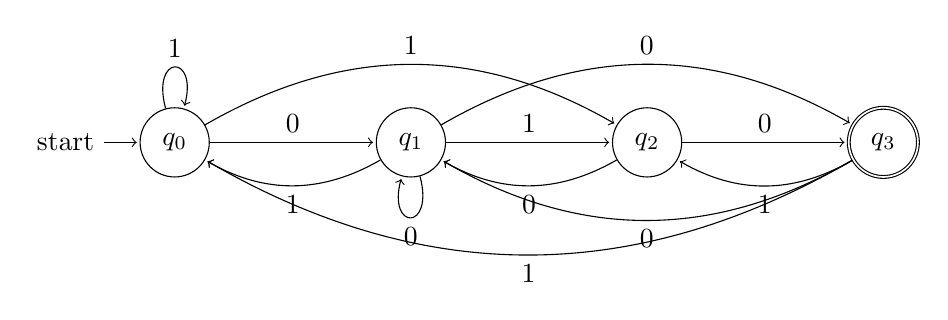
\begin{tikzpicture}[node distance=3cm,shorten >=1pt,auto]
\node[state,initial] 	(q_0)			{$q_0$};
\node[state]		(q_1)	[right of=q_0]	{$q_1$};
\node[state]		(q_2)	[right of=q_1]	{$q_2$};
\node[state,accepting]	(q_3)	[right of=q_2]	{$q_3$};
\path[->]		(q_0)	edge 			node	{$0$}		(q_1)
				edge [bend left]	node	{$1$}		(q_2)
				edge [loop above]	node	{$1$}		()
			(q_1)	edge [bend left]	node	{$1$}		(q_0)
				edge [loop below]	node	{$0$}		()
				edge [bend left]	node	{$0$}		(q_3)
				edge 			node	{$1$}		(q_2)
			(q_2)	edge [bend left]	node	{$0$}		(q_1)
				edge			node	{$0$}		(q_3)
			(q_3)	edge [bend left]	node	{$1$}		(q_0)
				edge [bend left]	node	{$1$}		(q_2)
				edge [bend left]	node	{$0$}		(q_1);
\end{tikzpicture}
\end{figure}
\end{center}

\item Potenzmengenkonstruktion
\begin{figure}[H]
\begin{center}
\begin{tabular}{l l | l | l}
 & & 0 & 1 \\
\hline
$q_0'$:&\{$q_0$\} & \{$q_1$\} & \{$q_0, q_2$\} \\
$q_1'$:& \{$q_1$\} & \{$q_1, q_3$\} & \{$q_0, q_2$\} \\
$q_2'$:& \{$q_0, q_2$\} & \{$q_1, q_3$\} & \{$q_0, q_2$\} \\
$q_3'$:& \{$q_1, q_3$\} & \{$q_0, q_1, q_2, q_3$\} & \{$q_0, q_2$\} \\
$q_4'$:& \{$q_0, q_1, q_2, q_3$\} & \{$q_0, q_1, q_2, q_3$\} & \{$q_0, q_2$\} \\

\end{tabular}
\end{center}
\end{figure}
\item Automat bisher (nach Umbennenung der Zustände):
\begin{figure}[H]
\begin{center}
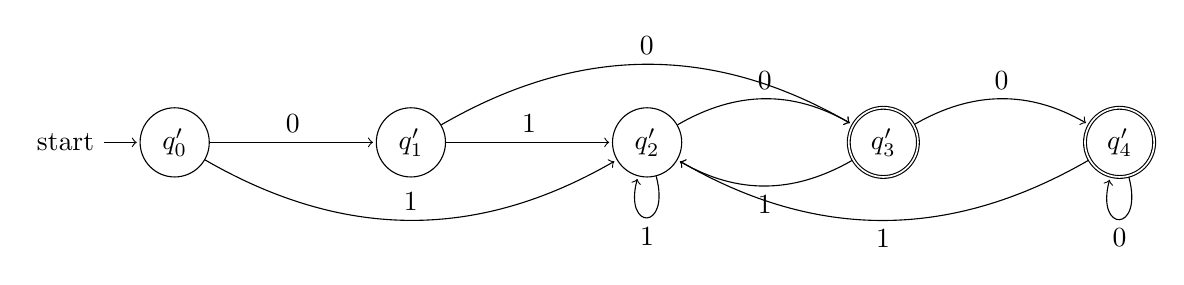
\begin{tikzpicture}[node distance=3cm,shorten >=1pt,auto]
\node[state,initial] 	(q_0)			{$q_0'$};
\node[state]		(q_1)	[right of=q_0]	{$q_1'$};
\node[state] 	  	(q_2)	[right of=q_1]	{$q_2'$};
\node[state,accepting]	(q_3)	[right of=q_2]	{$q_3'$};
\node[state,accepting]	(q_4)	[right of=q_3]	{$q_4'$};
\path[->]		(q_0)	edge 			node	{$0$}		(q_1)
				edge [bend right]	node	{$1$}		(q_2)
			(q_1)	edge [bend left]	node	{$0$}		(q_3)
				edge 			node	{$1$}		(q_2)
			(q_2)	edge [bend left]	node	{$0$}		(q_3)
				edge [loop below]	node	{$1$}		(q_2)
			(q_3)	edge [bend left]	node	{$0$}		(q_4)
				edge [bend left]	node	{$1$}		(q_2)
			(q_4)	edge [loop below]	node	{$0$}		(q_4)
				edge [bend left]	node	{$1$}		(q_2);
\end{tikzpicture}
\end{center}
\end{figure}
\item Minimierung
\begin{enumerate}
\item Trennung durch $\varepsilon$: \{$q_0', q_1', q_2'$\} \{$q_3', q_4'$\}
\item Trennung durch $1$: \{$q_0', q_1', q_2'$\} \{$q_3', q_4'$\}
\item Trennung durch $0$: \{$q_0'$\} \{$q_1', q_2'$\} \{$q_3', q_4'$\}
\item Keine weitere Trennung durch längere Zeugen: Abbruch
\end{enumerate}
\item Minimierter DEA:
\begin{figure}[H]
\begin{center}
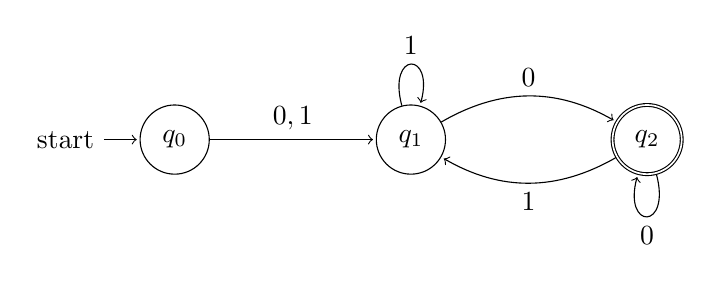
\begin{tikzpicture}[node distance=3cm,shorten >=1pt,auto]
\node[state,initial] 	(q_0)			{$q_0$};
\node[state]		(q_1)	[right of=q_0]	{$q_1$};
\node[state,accepting]	(q_2)	[right of=q_1]	{$q_2$};
\path[->]		(q_0)	edge 			node	{$0,1$}		(q_1)
			(q_1)	edge [loop above]	node	{$1$}		()
				edge [bend left]	node	{$0$}		(q_2)
			(q_2)	edge [bend left]	node	{$1$}		(q_1)
				edge [loop below]	node	{$0$}		();
\end{tikzpicture}
\end{center}
\end{figure}
\end{enumerate}
\item Nach 1. gibt es 3 Klassen. Finde also lediglich Repräsentanten. Etwa:
\begin{enumerate}
\item $[\varepsilon] = \{\varepsilon\}$
\item $[0] = \{0,1\}$
\item $[00] = \{0,1\}\{0,1\}^*0$
\end{enumerate}
\item $(0 \cup 1)(0 \cup 1)^*0$ erfüllt die Bedingung
\item Ja, Beweis etwa über strukturelle Induktion. %TODO?
\end{enumerate}
}{}
\section{Pumping Lemma}
\ifthenelse{\boolean{ex}}{
\subsection{Aufgaben}
Zeige oder Wiederlege die regulärität folgender Sprachen:
\begin{enumerate}
\item $\{a^ib^j | i \leq j\}$
\item $\{w | w\mbox{ enthält nicht die Zeichenkette } abc \mbox{ oder }cba\}$
\item $\{a^ib^j | i \geq j\}$
\item $\{www | w \in \Sigma^* \}$
\item $\{w | w\mbox{ enthält nicht genau zweimal }a\}$
\item $\{w | w\mbox{ ist kein Palindrom }\}$
\item Sei $\Sigma = \{0,1,+,=\}$ und $L = \{x=y+z | x,y,z \mbox{ Sind binäre Integer und }x = y + z\}$
\end{enumerate}
}{}
\ifthenelse{\boolean{sol}}{
\subsection{Lösungen}
\begin{enumerate}
\item Pumping 
\item Die Sprache ist regulär: Konstruktion eines NEA der die Sprache, die die Zeichenketten $abc$ oder $cba$ enthält ist trivial. Das Komplement ist also regulär.
\item nein
\item nein
\item ja
\item nein
\item nein
\end{enumerate}
}{}
\section{Turingmaschinen und Entscheidbarkeit}
\begin{enumerate}
\item Wieviele verschiedene Sprachen gibt es? Wie steht das im Verhältnis zu der Anzahl der Turingmaschinen? Kann man dadurch eine Aussage über die Existenz von nichtentscheidbaren Sprachen machen?
\item Schreibe jeweils eine Turingmaschine, die die folgenden Sprachen erkennt:
\begin{enumerate}
\item $\{a^ib^i\}$
\item $\{a^ib^j\ | i \leq j\}$
\item $\{w | w\mbox{ enthält nicht die Zeichenkette } abc \mbox{ oder }cba\}$
\item Sei $\Sigma = \{0,1,+,=\}$ und $L = \{x=y+z | x,y,z \}$
\end{enumerate}
\item Zeige, dass eine Sprache entscheidbar ist gdw. eine Turingmaschine existiert, die bei Eingabe eines Wortes der Sprache das Lexikografisch nächste Wort ausgibt.
\item Zeige, dass eine Sprache semientscheidbar ist gdw. eine Turingmaschine existiert, die bei Eingabe eines Wortes der Sprache, das nächste Wort der Sprache bezüglich einer festen Ordnung ausgibt.
\item Formuliere das Problem der Entscheidung ob ein Endlicher Automat und ein regulärer Ausdruck äquivalent sind als Sprache und zeige, dass diese Sprache entscheidbar ist.
\item Finde eine Lösung für folgendes PCP: $\{(ab,abab),(b,a),(aba,b),(aa,a)\}$
\item Zeige das eine TM die auf den Teil des Bandes, auf dem die Eingabe steht nicht schreiben kann, nur reguläre Sprachen erkennen kann.
\end{enumerate}
\section{Komplexitätsklassen}
\begin{enumerate}
\item Folgt aus $A \propto B$ und $B$ regulär, dass A auch regulär ist? 
\item Zeige: aus $A \propto co-A$ und $A$ semientscheidbar folgt, dass $A$ entscheidbar ist. Zeige auch: $A$ muss semientscheidbar sein durch Angabe einer Sprache $B$ mit $B \propto co-B$, aber $B$ nicht entscheidbar.
\item Gibt es eine unentscheidbare Teilmenge von $1^*$?
\item Zeige das $\mathcal{P}$ und $\mathcal{NP}$ jeweils unter Konkatenation und Vereinigung abgeschlossen sind. 
\item Zeige, dass wenn $\mathcal{P} = \mathcal{NP}$ gilt, dass ein polyzeit Algorithmus zum faktorisieren von Zahlen existiert.
\item Zeige, dass wenn $\mathcal{P} = \mathcal{NP}$ gilt, dass ein polyzeit Algorithmus zum finden der größten Clique in einem Graphen existiert
\item Sei DOPPEL-SAT $= \{\Phi | \Phi\mbox{ hat mindestens zwei erfüllende Belegungen}\}$, zeige das DOPPEL-SAT $\in \mathcal{NPC}$
\end{enumerate}
\end{document}
